% !TeX encoding = UTF-8
% !TeX spellcheck = es_ES
% !TeX root = WhatIs.tex
%!TEX root=WhatIs.tex

\documentclass[spanish]{DccDiyTools/DccDiyTools}
\usepackage[spanish]{babel}
\usepackage[
type={CC},
modifier={by-sa},
version={4.0},
]{doclicense}

\usepackage[]{DccDiyTools/DccDiyToolsPics}
\usepackage[]{DccDiyTools/DccDiyToolsComponentTables}


\title{What Is DCC DiY Tools}
\subtitle{Manifiesto de DCC DiY Tools}
\author{Daniel Vilas}
\date{Julio 2022}

\dbHeaderTitle{What Is DCC DiY Tools}
\dbType{M}
\dbDate{22}
\dbCode{002}
\dbStatus{Draft}
\dbVersion{0.1}
%\tikzset{
    pics/SmallBoard/.style={
      code = {
        % \draw [step=0.1,very thin, yellow] (-2,-1) grid (2,1);
        % \draw [step=0.5,very thin, red] (-2,-1) grid (2,1);
        % \draw [very thin, green] (-2,-1) grid (2,1);
        \node[inner sep=0pt] at (0,0)
        {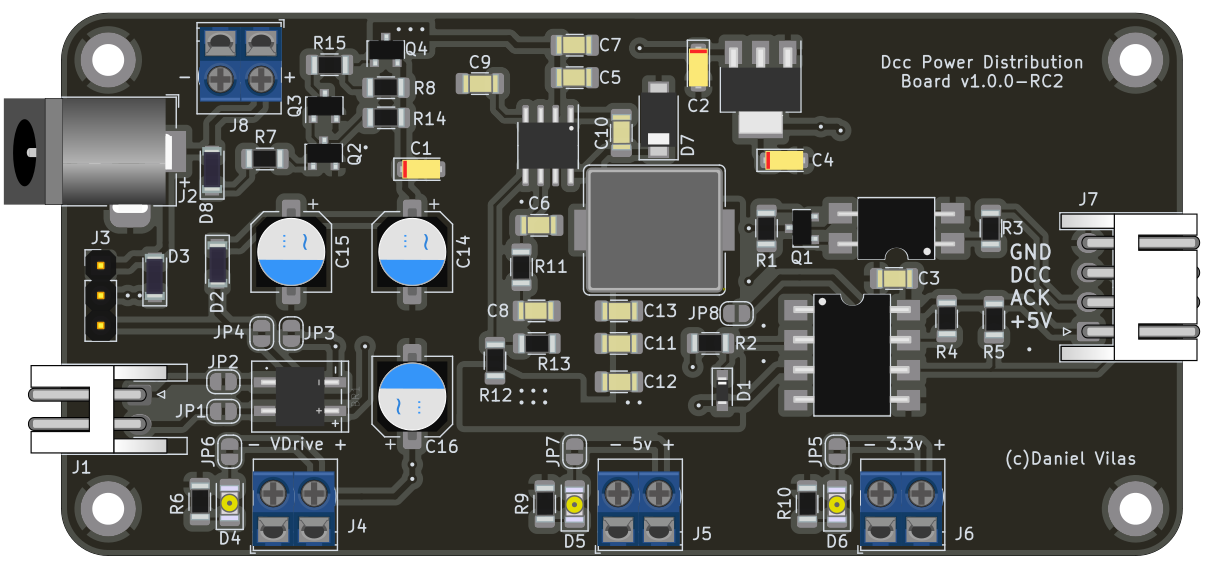
\includegraphics[scale=0.25]{images/front.png}};  


        \node[](-jack) at (-1.35,0.278) {};
        \node[](-terminal) at (-.8,0.65) {};
    }}
}

\tikzset{
    pics/WallAc/.style={
      code = {
    \begin{scope}[shift={(0.25,0)}]
        % \draw [step=0.1,very thin, yellow] (-2,-2) grid (2,2);
        % \draw [step=0.5,very thin, red] (-2,-2) grid (2,2);
        % \draw [very thin, green] (-2,-2) grid (2,2);
        % Mains lead
        \draw[line width=2pt,cap=round, lightgray] (0.05,-0.21) -- (0.05,-0.45);
        \draw[line width=2pt,cap=round, lightgray] (0.275,-0.21) -- (0.275,-0.45);
        % Relief and out cable
        \draw[line width=2pt,cap=round] (-0.5,0.25) -- (-1,0.25);
        \draw[line width=2pt,cap=round,black!75] (-0.55,0.35)--(-0.55,0.15);
        \draw[line width=2pt,cap=round,black!75] (-0.63,0.325)--(-0.63,0.175);
        \draw[line width=2pt,cap=round,black!75] (-0.71,0.3)--(-0.71,0.2);
        \draw[line width=2pt,cap=round,black!75] (-0.79,0.275)--(-0.79,0.225);
        \draw[line width=2pt,cap=round,black!75] (-0.87,0.275)--(-0.87,0.225);

        \draw[line width=2pt,rounded corners=1pt,fill=black!75] (-0.5,0) rectangle +(1,0.5);
        \draw[line width=2pt,rounded corners=1pt,fill=black!65] (-0.1,0) rectangle +(0.5,-0.2);
        % \draw[line width=2pt,cap=round, gray] (0.05,-0.21) -- (0.05,-0.45);
        % \draw[line width=2pt,cap=round,gray] (0.275,-0.21) -- (0.275,-0.45);

        \node[white,scale=0.5] at (0,0.25) {DC Wall};
        \node[](-jack) at (-1.1,0.25) {};
        \node[](-mains) at (.1625,-0.55) {};
    \end{scope}
    }}
}

\begin{document}
\maketitle
\newpage
\section{Introduccion}
% !TeX encoding = UTF-8
% !TeX spellcheck = es_ES
% !TeX root = CBus.tex
%!TEX root=CBus.tex
C-Bus es un standard LCB usado y promocionado por MERG\copyright. A bajo nivel utiliza un Bus CAN como transporte fisico de datos entre modulos (electronicos).

La idea de despligue es usar una topolgia de bus:
\begin{figure}[H]
    \centering
    \begin{tikzpicture}
        %\draw [very thin, green]  (-6,-3) grid (6,3);
        \node at (-6,3) [rectangle,draw,align=left] (ps) {Previous\\Segment};
        \node at (6,3) [rectangle,draw,align=left] (ns) {Next\\Segment};
        
        \node at (-2.75,0) [rectangle,draw,align=left] (d1) {Modulo 1};
        \node at (0,0) [rectangle,draw,align=left] (d2) {Modulo 2};
        \node at (2.75,0) [rectangle,draw,align=left] (d3) {Modulo ...};

        \draw [line width=2, blue] (-4,3) -- (-4,0) --(d1.west);
        \draw [line width=2, blue] (-1.25,3) -- (-1.25,0) --(d2.west);
        \draw [line width=2, blue] (1.5,3) -- (1.5,0) --(d3.west);

        \draw [line width=5] (ps.east) -- (ns.west);
    \end{tikzpicture}
    \caption{C-Bus Segmento}
    \label{fig:cBusSegment}
\end{figure}

Al final de un segmento puede haber otro segmento, un repetidor, un convertidor a Ethernet,\dots.
Desde el bus a los dispositivos es necesario tener un latiguillo.




\newpage
\section{Que es}
% !TeX encoding = UTF-8
% !TeX spellcheck = es_ES
% !TeX root = WhatIs.tex
%!TEX root=WhatIs.tex

En un principio, como la mayoria de los aficionados al tren en miniatura, la aventura empieza hace unos años con un ovalo de vias,
un transformador o mando analogico, una maquina y un par de vagones. El sistema digital DCC ya existe pero aun compite con otros\sidenote{Como "delta", MFX,\dots},
y aun no es muy accesible en terminos economicos. A su vez acaba de aparecer la platafoma de microntroladores Arduino que permite,
entre otras cosas, generar una señal PWM para controlar motores.

Armados con un con Arduino UNO, un Motor-Shield y un adapatador de corriente continua unos valientes comprueban que es posible
controlar la velocidad de un tren y su direccion digitalmente. A partir de esto ellos mismos se fabrican unos circuitos sencillos
para dar algo más de funcionalidad, como una placa que usa la corriente de accesorios del transformador analogico, un display
LCD de 20x02 caracteres, una placa de proteccion ante corto circuitos,\dots

Con el tiempo el sistema DCC se hace más accesible, y ademas, la lista de modulos creados se amplia a cosas DCC, y a su vez los estos son más
genericos y reutilizables\sidenote{Sin o con pocas modificaciones}. Han pasado de ser algo muy particular para los problemas de
una maqueta, a ser herramientas que puden ser usadas en todas las maquetas.

En un momento dado se da la posibilidad de hacer una nueva maqueta y se toma la decision de normalizar\sidenote{O standarizar,
como se prefiera decir} una serie de componentes(Conectores, cables, etc\dots) y con ella de documentar los modulos que se hagan
como si fuera un producto comercial. Ha nacido DCC DiY Tools.
\begin{itemize}
    \item \textit{DCC DiY Tools} es una declaracion de intenciones. De la intencion de hacer las cosas bien.
    \item Hacer los modulos reutilizables y adaptables a cualquier maqueta, como un producto de una empresa
    \item Con calidad y repetibilidad. Pudiendo garantizar que se cumplen las especificaciones. 
    \item Siguiendo una normativa propia, como por ejemplo de conectores, para que los modulos sean similares
    \item Con los documentos necesarios equivalentes a los que se necesitan en una empresa, tales como manuales de usuario, de 
    analisis y diseño, esquematicos, \dots
    \item Basado en la descripcion de Open Source HardWare, o OSHW, con toda la documentacion abierta y libre. Ya no solo la 
    minima requerida por la OSHW, si no de las decisiones tomadas y su razon.
    \item Seran educativos. O que puedan servir\sidenote{Aunque sea de lo que no hay que hacer} para entender las cosas.
    \item Un conjunto de repositorios git o similar.
\end{itemize}

En resumen \textit{Dcc DiY Tools} es un repositorio de informacion abierta, lo mas completa posible, de modulos OSHW usables
en maquetas de tren, tanto digitales, como analogicas.

Al ser más inforamacion que otra cosa, la licencia y la garantia de los productos manufacturados es la definida por OSHW, 
que se puede resumir\sidenote{Mas mal que bien} en  "<haz lo que quieras, sin ninguna garantia">, ver el apartado de
garantia y licencia para una informacion detallada.

\subsection{¿Que no es?}
DCC DiY Tools \textbf{no} es una empresa, ni una linea de productos, ni una tienda ni nada mas que un sitio de documentacion. 
Tampoco es un sitio web con una comunidad\sidenote{Ojala se convierta en ello.} que pueda dar soporte rapido\sidenote{Mientras
 tanto se dara lo que se pueda}.
En realidad es una persona intentando documentar sus circuitos de tal forma que les puedan servir a otros.
\end{document}